\documentclass[11pt,letterpaper]{article}
\usepackage[margin=0.6in]{geometry}
\usepackage{amsmath,amssymb}
\usepackage{tikz}
\usetikzlibrary{arrows.meta,positioning}
\usepackage{xcolor}
\usepackage{fontawesome5}
\usepackage{tcolorbox}
\usepackage{multicol}
\usepackage{enumitem}
\usepackage{hyperref}

\definecolor{primaryblue}{RGB}{41, 98, 255}
\definecolor{accentgreen}{RGB}{0, 150, 136}
\definecolor{warnorange}{RGB}{255, 152, 0}
\definecolor{lightgray}{RGB}{245, 245, 245}

\tcbset{
    conceptbox/.style={colback=primaryblue!5, colframe=primaryblue, boxrule=1pt, arc=3pt, left=5pt, right=5pt, top=5pt, bottom=5pt},
    formulabox/.style={colback=lightgray, colframe=gray!50, boxrule=0.5pt, arc=2pt, left=5pt, right=5pt, top=3pt, bottom=3pt},
    warningbox/.style={colback=warnorange!10, colframe=warnorange, boxrule=1pt, arc=3pt, left=5pt, right=5pt, top=5pt, bottom=5pt},
    appbox/.style={colback=accentgreen!5, colframe=accentgreen, boxrule=1pt, arc=3pt, left=5pt, right=5pt, top=5pt, bottom=5pt}
}

\pagestyle{empty}
\setlength{\parindent}{0pt}
\setlist[itemize]{leftmargin=*, itemsep=1pt, topsep=2pt}

\begin{document}

\begin{center}
{\LARGE\bfseries\color{primaryblue} Chapter 5: Optimization Basics}\\[3pt]
{\large Gradient Descent, Convexity, and Convergence}
\end{center}
\vspace{-5pt}
\hrule height 2pt
\vspace{8pt}

\begin{multicols}{2}

\begin{tcolorbox}[conceptbox, title={\faLightbulb\ Key Concepts}]
\begin{itemize}
    \item \textbf{Gradient Descent}: Move opposite to gradient
    \item \textbf{Learning Rate}: Step size $\eta$ --- critical hyperparameter
    \item \textbf{Convex Function}: Single global minimum guaranteed
    \item \textbf{Local vs Global Minima}: Initialization matters!
    \item \textbf{Saddle Points}: Gradient = 0, but not minimum
\end{itemize}
\end{tcolorbox}

\begin{tcolorbox}[formulabox, title={\faCalculator\ Core Formulas}]
\textbf{Gradient Descent Update:}
\[ \mathbf{x}_{t+1} = \mathbf{x}_t - \eta \nabla f(\mathbf{x}_t) \]

\textbf{Convexity Condition:}
\[ f(\lambda x + (1-\lambda)y) \leq \lambda f(x) + (1-\lambda)f(y) \]

\textbf{First-Order Optimality:}
\[ \nabla f(\mathbf{x}^*) = \mathbf{0} \]

\textbf{Second-Order (minimum):}
\[ \nabla^2 f(\mathbf{x}^*) \succ 0 \text{ (positive definite)} \]
\end{tcolorbox}

\columnbreak

\begin{center}
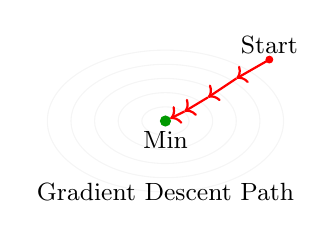
\begin{tikzpicture}[scale=0.6]
    % Contour plot simulation
    \draw[lightgray] (0,0) ellipse (2.5 and 1.5);
    \draw[lightgray] (0,0) ellipse (2 and 1.2);
    \draw[lightgray] (0,0) ellipse (1.5 and 0.9);
    \draw[lightgray] (0,0) ellipse (1 and 0.6);
    \draw[lightgray] (0,0) ellipse (0.5 and 0.3);

    % GD path
    \filldraw[red] (2.2, 1.3) circle (2pt);
    \draw[->,red,thick] (2.2,1.3) -- (1.5,0.9);
    \draw[->,red,thick] (1.5,0.9) -- (0.9,0.5);
    \draw[->,red,thick] (0.9,0.5) -- (0.4,0.2);
    \draw[->,red,thick] (0.4,0.2) -- (0.1,0.05);
    \filldraw[green!60!black] (0,0) circle (3pt);

    \node at (2.2,1.6) {\small Start};
    \node at (0,-0.4) {\small Min};
    \node at (0,-1.5) {\small Gradient Descent Path};
\end{tikzpicture}
\end{center}

\begin{tcolorbox}[appbox, title={\faRobot\ ML Applications}]
\begin{itemize}
    \item \textbf{Training Neural Networks}: GD on loss function
    \item \textbf{Learning Rate Schedules}: Decay over time
    \item \textbf{Momentum}: Accelerate through flat regions
    \item \textbf{Adam}: Adaptive learning rates per parameter
\end{itemize}
\end{tcolorbox}

\begin{tcolorbox}[warningbox, title={\faExclamationTriangle\ Common Pitfalls}]
\begin{itemize}
    \item Learning rate too high $\Rightarrow$ \textbf{divergence}
    \item Learning rate too low $\Rightarrow$ \textbf{slow convergence}
    \item \textbf{Saddle points} slow down training in high dimensions
    \item Non-convex loss: different inits $\Rightarrow$ different results
\end{itemize}
\end{tcolorbox}

\end{multicols}

\vspace{5pt}
\hrule
\vspace{5pt}

\begin{center}
\faGithub\ \textbf{Notebook}: \url{https://github.com/vijaygwu/math-powers-ai/blob/main/notebooks/ch05_optimization.ipynb}
\end{center}

\end{document}
